\section{Evaluation} \label{sec:evaluation}





Our evaluation machines include nine RDMA-enabled, Dell R430 servers as \paxos 
replicas. Each server has Linux 3.16.0, 2.6 GHz Intel Xeon CPU with 24 
hyper-threading cores, 64GB memory, and 1TB SSD. All NICs are Mellanox 
ConnectX-3 Pro 40Gbps connected with Infiniband~\cite{infiniband}. 
The \v{ping} latency between every two replicas is 84 \us (the IPoIB 
round-trip latency).
%
% through a Dell S6000 high-performance switch with 32 40Gpbs ports.

Our evaluation machines also include one Dell R320 server for client programs. 
It has Linux 3.16.0, 2.2GHz Intel Xeon 12 hyper-threading cores, 32GB memory, 
and 160GB SSD. To mitigate latency of client requests, this client machine is 
located at the same LAN as the RDMA replicas with a 1Gbps NIC. The average 
\v{ping} latency between this machine and a RDMA replica is 250 \us. Note that 
which machines to hold clients do not affect any \paxos protocol's consensus 
latency (it is only affected by the RDMA network among replicas).

We compared \xxx with five popular, open source \paxos-compatible 
implementations,
including four TCP/IP-based ones (\libpaxos~\cite{libpaxos},
\zookeeper~\cite{zookeeper}, \crane~\cite{crane:sosp15} and
\spaxos~\cite{spaxos:srds12}) and an RDMA-based one 
(\dare~\cite{dare:hpdc15}). \spaxos is designed to achieve scalable throughput 
when more replicas are added. 

We evaluated \xxx on \nprog widely used or studied server programs, including
\nkvprog key-value stores \redis, \memcached, \ssdb, \mongodb; \mysql, a SQL
server; \clamav, an anti-virus server that scans files and delete malicious ones;
\mediatomb, a multimedia storage server that stores and transcodes video and
audio files; \openldap, an LDAP server; \calvin, a widely studied transactional
database system. All these programs are multithreaded except \redis (but it can 
serve concurrent requests via Libevent). These servers all update or store 
important data and files, thus the strong \paxos fault-tolerance is especially 
attractive to these programs.


% Benchmarks table.
Table~\ref{tab:benchmarks} introduces the benchmarks and workloads we used. We 
used the protocol or program developers' own performance benchmarks or popular 
third-party benchmarks. For benchmark workload settings, we used the 
benchmarks' default workloads whenever available. To perform a stress testing 
on \xxx's input consensus protocol, we chose workloads with significant 
portions of writes, because write operations often contain more input bytes 
than reads (\eg, a key-value SET operation contains more bytes than a GET).

\begin{table}[h]
\footnotesize
\centering
\vspace{-.1in}
\begin{tabular}{lrr}
{\bf Program} & {\bf Benchmark} & {\bf Workload/input description}\\
\hline\\[-2.3ex]
\clamav & clamscan~\cite{clamscan}  & Files in \v{/lib} from a replica \\
\mediatomb & ApacheBench~\cite{apachebench}  & Transcoding videos\\
\memcached & mcperf~\cite{mcperf}  & 50\% set, 50\% get operations\\
\mongodb & YCSB~\cite{ycsb}  & Insert operations\\
\mysql & Sysbench~\cite{sysbench}  & SQL transactions\\
\openldap & Self  & LDAP queries\\
\redis & Self  & 50\% set, 50\% get operations\\
\ssdb & Self  & Eleven operation types\\
\calvin & Self  & SQL transactions\\
\end{tabular}

\caption{{\em Benchmarks and workloads.} ``Self" in the Benchmark column means
we used a program's own performance benchmark program. Workloads are all
concurrent.}
\vspace{-.05in}
\label{tab:benchmarks}
\end{table}


% evaluation metric. client benchmarks all run in LAN, average latency
The rest of this section focuses on these questions:

\begin{tightenum}

\item[\S\ref{sec:eval-traditional}:] How does \xxx performance compare
to TCP/IP-based \paxos protocols?

\item[\S\ref{sec:eval-dare}:] How does \xxx performance compare
to \dare?

\item[\S\ref{sec:overhead}:] What is the performance overhead of running \xxx
with server programs? How does it scale with the number of concurrent 
requests?

% \item[\S\ref{sec:scalability}:] How scalable is \xxx on different replica group
% sizes?

\item[\S\ref{sec:robust}:] How fast is \xxx on handling checkpoints and
electing a new leader?

% \item[\S\ref{sec:race}:] If some \xxx users care about data races much, how
% does \xxx tolerate the slowdown of data race detector by deploying it on a
% replica?

% \item[\S\ref{sec:lesson}:] What practical lessons have we learnt during the
% case study on these server programs with \xxx?

\end{tightenum}





\subsection{Comparing with TCP/IP-based \paxos}
\label{sec:eval-traditional}

A common practice in 
\paxos evaluation~\cite{dare:hpdc15,nopaxos:osdi16}, when comparing \xxx with 
other \paxos protocols, we ran \xxx with a popular key value store \redis.  
To stress \xxx on our 24-core machines, we spawned 24 concurrent requests for 
all six protocols, a common high concurrent value in prior 
evaluation~\cite{zookeeper,crane:sosp15,rex:eurosys14}. Our evaluation also 
showed that most server programs reached peak throughput before 16 requests 
(\S\ref{sec:overhead}).

% We compared \xxx with four TCP/IP-based protocols, \libpaxos~\cite{libpaxos},
% \zookeeper~\cite{zookeeper}, \crane~\cite{crane:sosp15} and
% \spaxos~\cite{spaxos:srds12}. 

All four TCP/IP-based protocols were run on IPoIB (\S\ref{sec:rdma}). 
Figure~\ref{fig:scalability} shows that the consensus latency of three 
traditional protocols increased almost linearly to the number of replicas 
(except \spaxos). \spaxos batches requests from replicas and invokes consensus 
when the batch is full. More replicas can take shorter time to form a batch, so 
\spaxos incurred a slightly better consensus latency with more replicas. 
Nevertheless, its latency was always over 600 \us. \xxx's consensus latency 
outperforms these four protocols by \comptradlow to \comptradhigh.

% \spaxos batch requests from replicas and it only invokes 
% consensus when a fixed batch is full. More replicas will make this batch be 
% full more quickly, so \spaxos incurred slightly better latency at 
% more nodes. 


To understand the scalability bottleneck in these four protocols, we spawned 
only one client and inspected the micro events in their protocols 
(Table~\ref{tab:traditional-latency}). From three to nine replicas, the 
consensus latency (the ``Latency" column) of these protocols increased more 
gently than that on 24 concurrent clients. For instance, when the number of 
replicas increased from three to nine, \zookeeper latency increased by 30.3\% 
with one client; this latency increased by 168.3\% with 24 clients 
(Figure~\ref{fig:scalability}). This indicates that concurrent consensus 
requests are the major scalability bottleneck for these protocols.

Specifically, three protocols had scalable latency on the arrival of their 
first consensus reply (the ``First" column), which implies that network is not 
saturate. \libpaxos is an exception because its two-round protocol consumed 
much bandwidth. However, there is a big gap between the arrival of the first 
consensus reply and the ``majority" reply (the ``Major" column). Given that the 
replies' CPU processing time was small (the ``Process" column), we can see that 
various systems layers, including OS kernels, network libraries, and 
language runtimes (\eg, JVM), are another major scalable bottleneck (the ``Sys" 
column). This indicates that RDMA is useful on bypassing these systems layers.

Note that on three replicas, \libpaxos and \crane's proposing 
leader and acceptors are in different threads, so they two had different 
``First" and ``Major" arrival times. \crane and \spaxos's proposing 
leader itself is just an acceptor, so they two had same ``First" and ``Major" 
arrival times (\ie, their ``Sys" times were 0).

% We compared \xxx with \calvin's SMR system because \calvin's input consensus
% uses \zookeeper, one of the most widely used coordination service built on
% TCP/IP. To conduct a fair comparison, we ran \calvin's own transactional
% database server in \xxx as the server program, and we compared throughputs and
% the consensus latency with \calvin's consensus protocol \zookeeper.

% As shown in Table~\ref{tab:compare}, \calvin's \zookeeper replication achieved
% 19.9K transactions/s with a 511.9 \us consensus latency. \xxx achieved 18.9K
% transactions/s with a 19.5 \us consensus latency. The throughput in \calvin
% was 5.3\% higher than that in \xxx because \calvin puts transactions in a
% batch with a 10 \ms timeout, it then invokes \zookeeper for consensus on
% this batch. The average number of bytes in \calvin's batches is 18.8KB, and
% the average number of input bytes in each \xxx consensus (one for each \myread
% call) is 128 bytes. Batching helps \calvin achieve good throughput. \xxx
% currently has not incorporated a batching technique because its latency is
% already reasonable (\S\ref{sec:overhead}).
% 
% Notably, \xxx's consensus latency was 40.1X faster than \zookeeper's mainly due
% to \xxx's RDMA-accelerated consensus protocol, although we ran \calvin's
% \zookeeper consensus on IPoIB. A prior SMR evaluation~\cite{dare:hpdc15} also
% reports a similar 320 \us consensus latency in \zookeeper. Two other recent SMR
% systems Crane~\cite{crane:sosp15} and Rex~\cite{rex:eurosys14} may incur
% similar
% consensus latency as \zookeeper's because all their consensus protocols are
% based on TCP/IP. Overall, this \xxx-\calvin comparison suggests that \calvin
% will be better if clients prefer high throughput, and \xxx will be better if
% clients demand short latency.
% TBD: rerun \redis micro events; it is too small, so we can not use it here.

\begin{table}[h]
\footnotesize
\centering
\vspace{.05in}
\begin{tabular}{lrrrrr}
{\bf Proto-\#Rep} & {\bf Latency} & {\bf First} & {\bf Major} & {\bf
Process}
& {\bf Sys}\\
\hline\\[-2.3ex]
\libpaxos-3 & 81.6 & 74.0  & 81.6 & 2.5 & 5.1\\
\libpaxos-9 & 208.3 & 145.0  & 208.3 & 12.0 & 51.3\\

\hline\\[-2.3ex]
\zookeeper-3 & 99.0 & 67.0  & 99.0 & 0.84 & 31.2\\
\zookeeper-9 & 129.0 & 76.0  & 128.0 & 3.6 & 49.4\\

\hline\\[-2.3ex]
\crane-3 & 78.0 & 69.0  & 69.0 & 13.0 & 0\\
\crane-9 & 148.0 & 83.0  & 142.0 & 30.0 & 35.0\\

\hline\\[-2.3ex]
\spaxos-3 & 865.1 & 846.0  & 846.0 & 20.0 & 0\\
\spaxos-9 & 739.1 & 545.0  & 731.0 & 35.0 & 159.1\\

\end{tabular}
\vspace{-.05in}
\caption{{\em Performance breakdown of TCP/IP-based \paxos protocols 
with only one client.} The ``Proto-\#Rep" column means the protocol name 
and replica group size; ``Latency" means the consensus latency; ``First" means 
the latency of its first consensus reply; ``Major" means the
latency of its the majority reply; ``Process" means time spent in
processing all replies; and ``Sys" means time spent in systems (OS
kernel, network libraries, and JVM) between the ``First" and the ``Major" 
reply. All times are in \us.}
\label{tab:traditional-latency}
\vspace{-.2in}
\end{table}

\subsection{Comparing with \dare}
\label{sec:eval-dare}

\begin{figure}[t]
\centering
\vspace{-.10in}
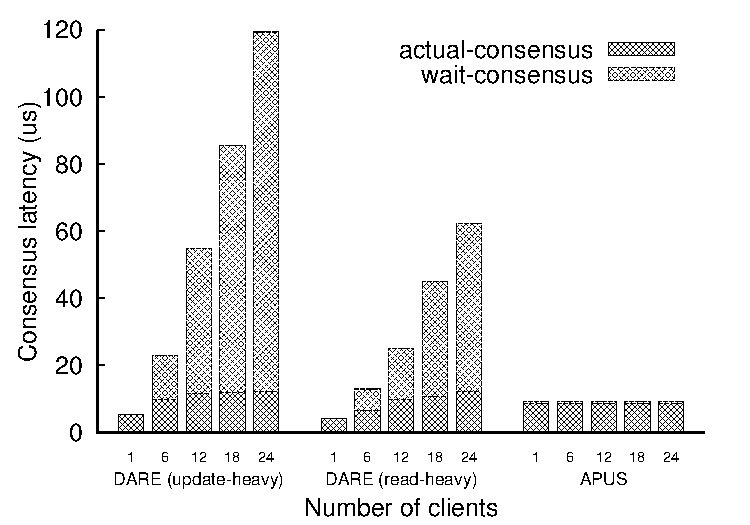
\includegraphics[width=.4\textwidth]{figures/server-processing-compare}
\vspace{-.1in}
\caption{{\em Consensus latency and its breakdown of \xxx and \dare.} The 
number of replicas is seven. Consensus latency contains two parts: 
``Wait-time" means the duration between the time a request being received by a 
server program and the time a consensus for this request starts. 
``Consensus-time" means the actual duration for consensus.}
\label{fig:compare}
\vspace{-.25in}
\end{figure}


\begin{figure*}[t]
\centering
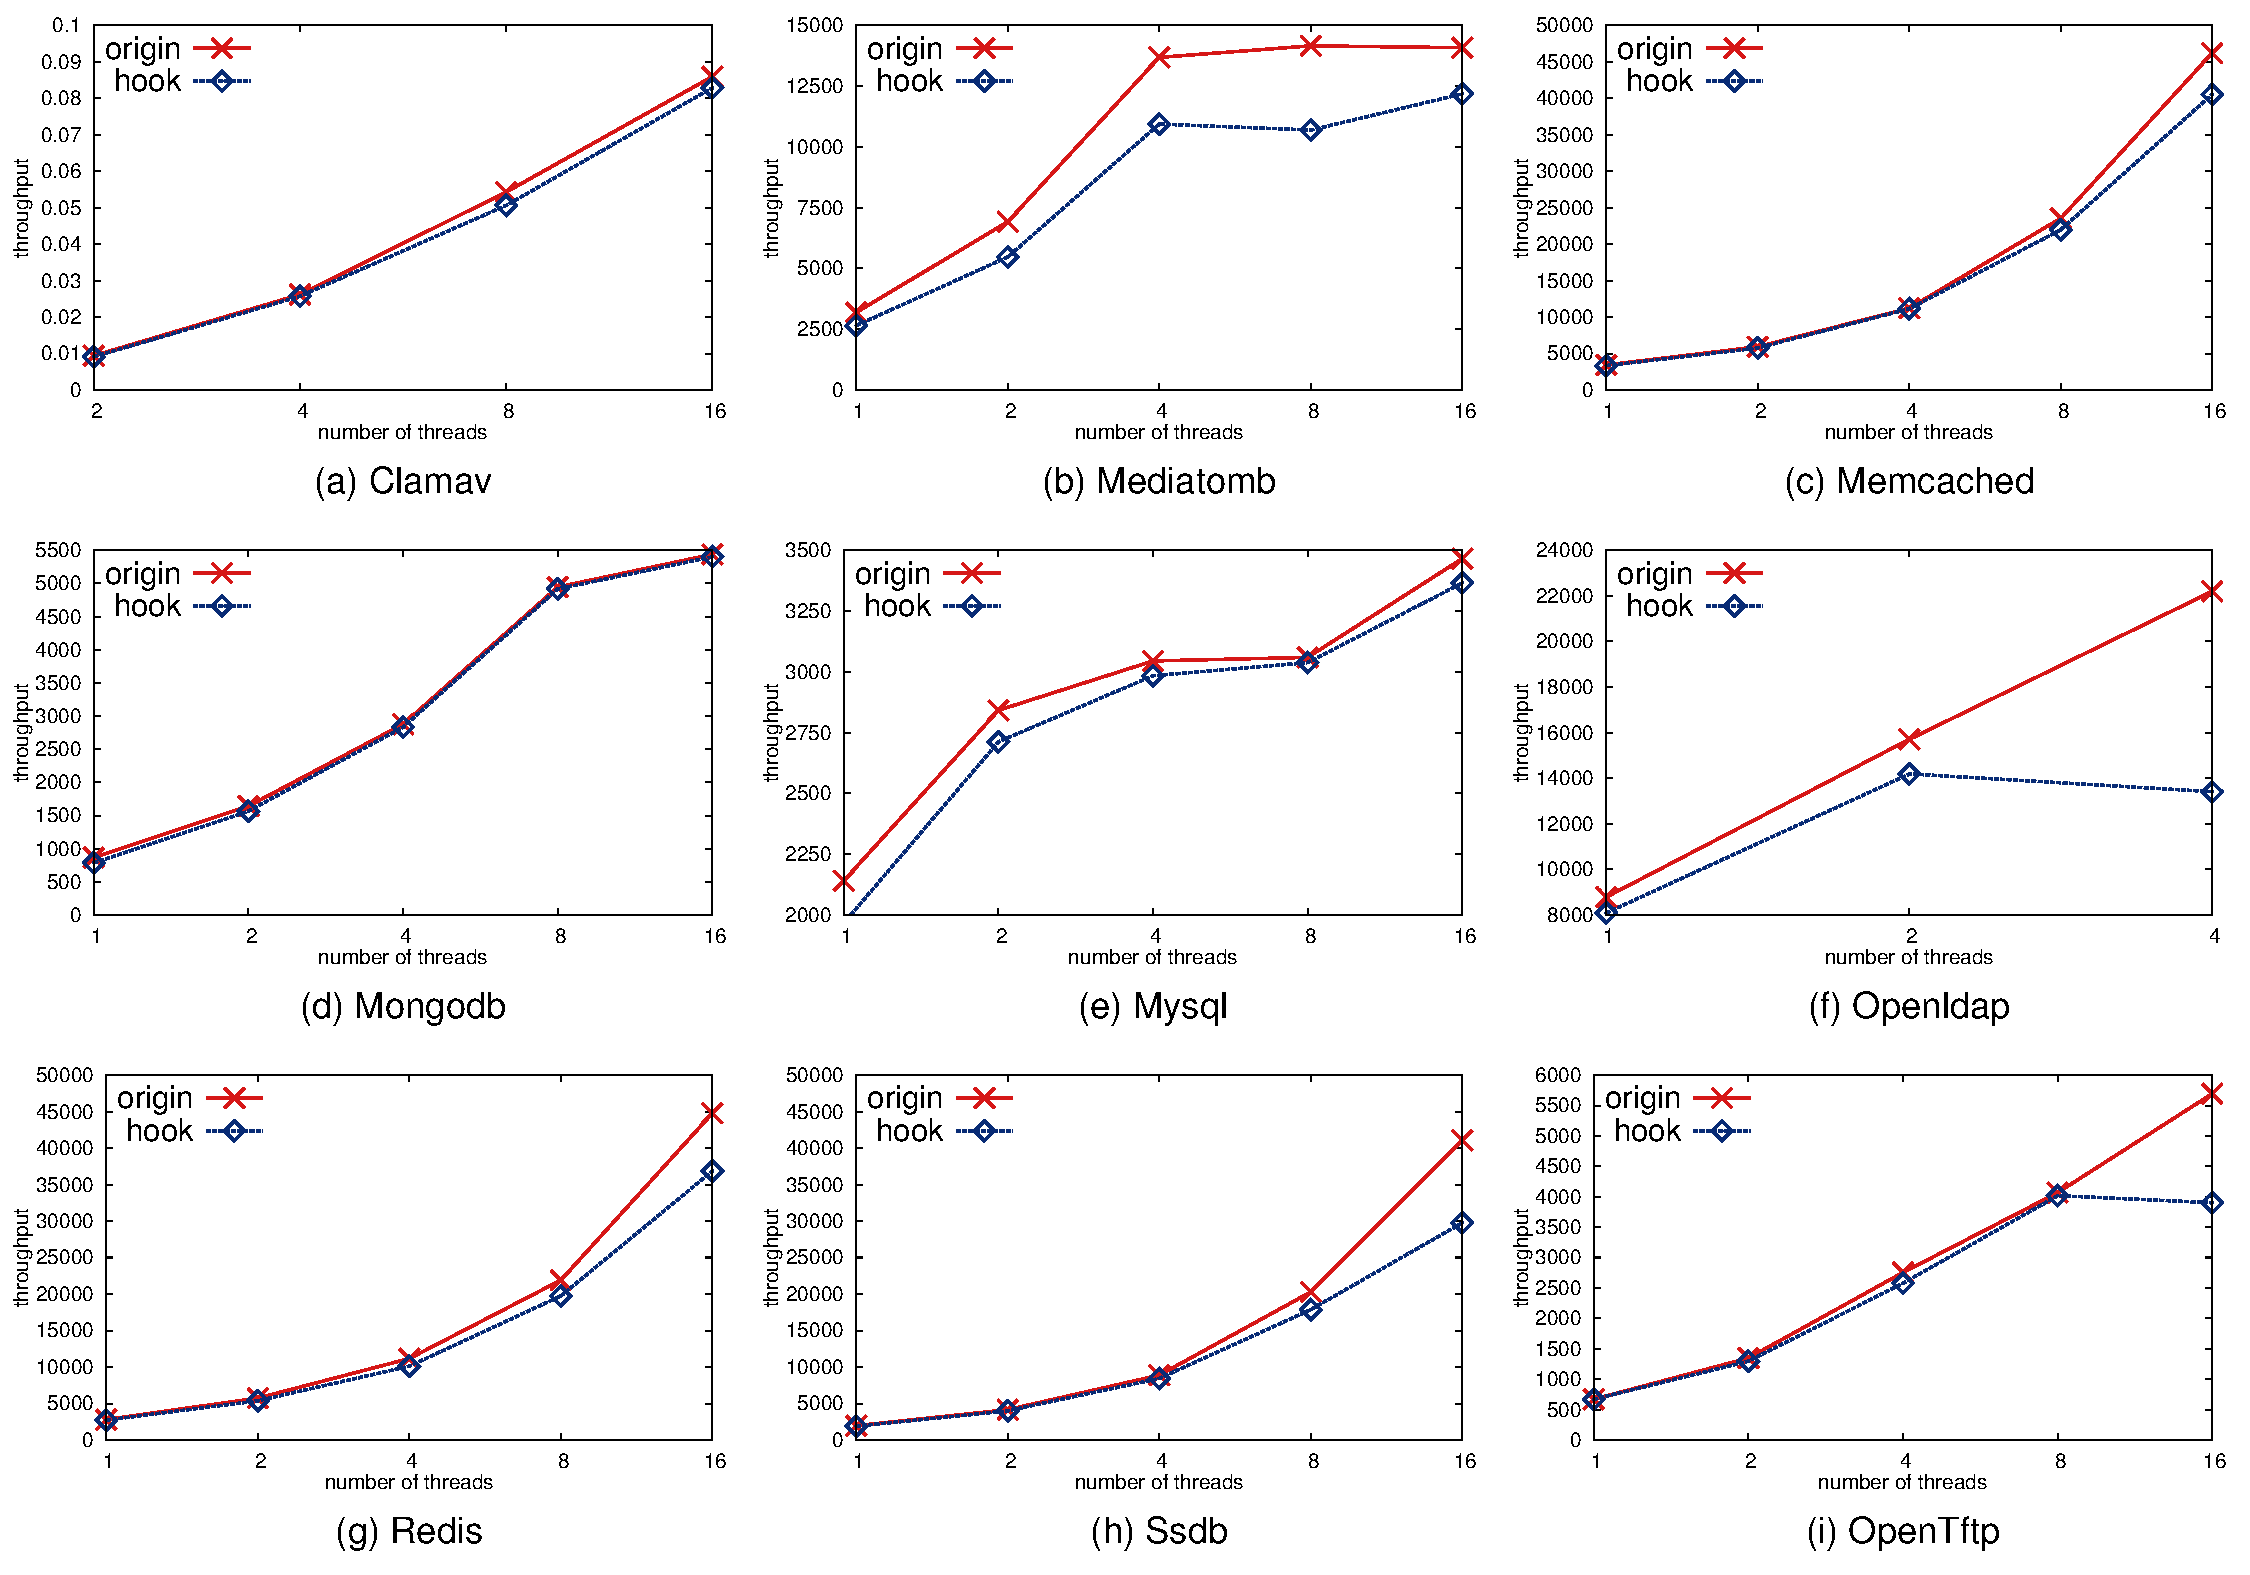
\includegraphics[width=0.9\textwidth]{figures/throughput}
\vspace{-.10in}
\caption{\small {\em \xxx throughput compared to the unreplicated
execution.}}
\vspace{-.20in}
\label{fig:tput}
\end{figure*}

We compared \xxx and \dare~\cite{dare:hpdc15} on key-value servers with same 
requests. \xxx ran a widely used one, \redis; \dare supported a 335-line, 
RDMA-based key-value server written by their authors. To thoroughly analyze 
their latency with scalability, we ran up to seven replicas and 24 clients. 
% Since our RDMA NIC bandwidth is 40Gpbs, our network were not s while 
% running several replicas on one machine: when changing replica group size from 9 
% to 105, an RDMA round-trip increased from 2.6$\sim$4.4 \us.

Figure~\ref{fig:compare} shows the consensus latency of \xxx 
and \dare on seven replicas with randomly arriving, update-heavy (50\% SETs and 
50\% GETs) and read-heavy (10\% SETs and 90\% GETs) workloads. \dare 
performance on these two workloads were different because it handles GETs with 
only one consensus round~\cite{dare:hpdc15}. \xxx handles all requests with the 
same protocol. When there was only one client, \xxx was slightly slower than 
\dare because \dare does not store inputs persistently. On 6 to 24 requests, 
\xxx was \fasterDARElow to \fasterDAREhigh faster than \dare due to two reasons.

First, \xxx is a one-round protocol and \dare is a two-round protocol (for 
SETs), so \dare's actual consensus time was \fasterDAREconsensusonly higher than 
\xxx. Even comparing \dare's read-heavy workloads (one-round for GETs) with 
\xxx on more concurrent requests, \xxx's actual consensus time was still 
slightly faster than \dare's because \xxx's protocol avoids expensive ACK 
pollings (\S\ref{sec:rdma}).

Second, \dare's second consensus round updates a global variable in remote 
backups, which serializes ongoing consensus requests (\S\ref{sec:compare}). 
Although \dare compensates this limitation by batching same SET or GET types, 
the randomly arrival of requests often make batches small, causing a large 
wait duration (a new batch can not start consensus until prior batches 
reach consensus). \dare's evaluation~\cite{dare:hpdc15} confirmed a high 
wait duration: with three replicas and nine concurrent clients, \dare's 
throughput on real-world inspired workloads (50\% SET and 50\% GET arriving 
randomly) was 43.5\% lower than that on 100\% SET workloads. \dare's 
evaluation also showed that its throughput dropped by 30.1\% when the number of 
replicas increased from three to seven.

Overall, these results indicate that \dare is better on smaller number of 
concurrent requests and replicas (\eg, 
leader election~\cite{chubby:osdi,zookeeper}), and \xxx is better on larger 
number of concurrent requests or replicas (\eg, replicating server 
programs~\cite{rex:eurosys14,crane:sosp15}).

% \xxx and \dare 
% achieved similar latency at three replicas, and \xxx was much faster than \dare 
% on more replicas. Their difference was 2.5x$\sim$3.3x on over 33 replicas. When 
% changing replica group size from 3 to 105 (a 35x increase), \xxx's consensus 
% latency merely increased by \xxxscalability, and \dare increased by 
% \darescalability.
% This workload represents 
% real-world applications such as an advertisement 
% log that records recent user activities~\cite{dare:hpdc15}. 

% \xxx scales better than \dare due to two main reasons. First, in a protocol 
% level, \xxx's protocol carefully separate the RDMA workloads across leader and 
% backups, and it is a one-round protocol (\S\ref{sec:normal}). \dare lets its 
% leader do all the consensus work and backups do nothing, and it is a two-round 
% protocol (\S\ref{sec:compare}). Therefore, \dare involves approximately 2x more 
% RDMA communications than \xxx.
% 
% Second, in an RDMA communication primitive level, \xxx lets all replicas 
% receive consensus messages on their bare, local memory. \dare frequently polls 
% RDMA ACKs from a RDMA Completion Queue (CQ) in each consensus round. An ACK 
% polling or insertion operation on the CQ involves synchronization between 
% RDMA NICs among replicas. We found that \dare's ACK mechanism is 
% already highly optimized with a global CQ (it can poll more ACKs at 
% one time). However, we found that ACKs arrived randomly, and each 
% polling in \dare took up to 0.042 \us (\S\ref{sec:background}). The 
% number of ACK pollings in \dare is linear to replica group 
% size (\S\ref{sec:compare}), causing a linearly increased consensus latency.

% \xxx does the same consensus round on all types of requests. \dare has two 
% special techniques on GET requests. First, it batches GET requests for 
% consensus, which may improve throughput but aggravate latency. Second, \dare's 
% GET requests only involve one-round consensus (it does RDMA reads to fetch all 
% replicas' \paxos view IDs~\cite{paxos:practical} and check if a majority of 
% them match the leader's). We also ran \dare with a read-heavy workload 
% (Table~\ref{tab:rdma-latency}) and its consensus latency was about 50\% 
% slower than \xxx on over 33 replica groups. Note that \xxx is a durable 
% protocol, and \dare is a volatile protocol. Overall, we considered \xxx faster 
% and more scalable than \dare.

% \begin{table}[h]
% \footnotesize
% \centering
% % \vspace{-.1in}
% \begin{tabular}{lrrrrr}
% 
% {\bf \# Replicas} & {\bf 3} & {\bf 9}\\
% \hline\\[-2.3ex]
% \xxx (update-heavy) & 8.2 & 8.8 & 13.0 & 20.3 & 31.6 \\
% 
% \hline\\[-2.3ex]
% \dare (update-heavy) & 8.8 & 12.0  & 32.5 & 64.0 & 102.5 \\
% 
% \hline\\[-2.3ex]
% \dare (read-heavy) & 5.8 & 7.2 & 16.8 & 29.2 & 45.1 \\
% 
% \end{tabular}
% \vspace{-.05in}
% \caption{{\em Consensus latency of \xxx and \dare.} The update-heavy workload 
% consist of 50\% SETs. The read-heavy workload consist of 10\% SETs.}
% \label{tab:rdma-latency}
% \vspace{-.2in}
% \end{table}

% Table~\ref{tab:consensus-latency} shows the Scalability results. Given the same
% workload, \xxx's five-replica setting had a 17.9K requests/s and 10.1
% \us consensus latency, and its seven-replica setting had a 17.4K requests/s and
% 11.0 \us consensus latency. Compared to the three-replica setting, \xxx
% achieved a similar consensus latency from three to seven replicas, because a
% \xxx consensus latency mainly contains two SSD stores and one WRITE round-trip
% (see Table~\ref{tab:consensus-latency}).
% 
% We didn't consider these initial scalability results general; we found them
% promising. Given that each RDMA NIC hardware port supports up to 16 outbound
% RDMA WRITEs with peak performance~\cite{herd:sigcomm14}, and our NIC has dual
% ports, we anticipate that our algorithm may scale up to around 32 replicas
% under current hardware techniques. We plan to buy more servers and verify
% whether \xxx's scalability is bounded by RDMA NIC capacity. \S\ref{sec:comp}


\subsection{Performance Overhead} \label{sec:overhead}

% \begin{figure*}[t]
% \centering
% 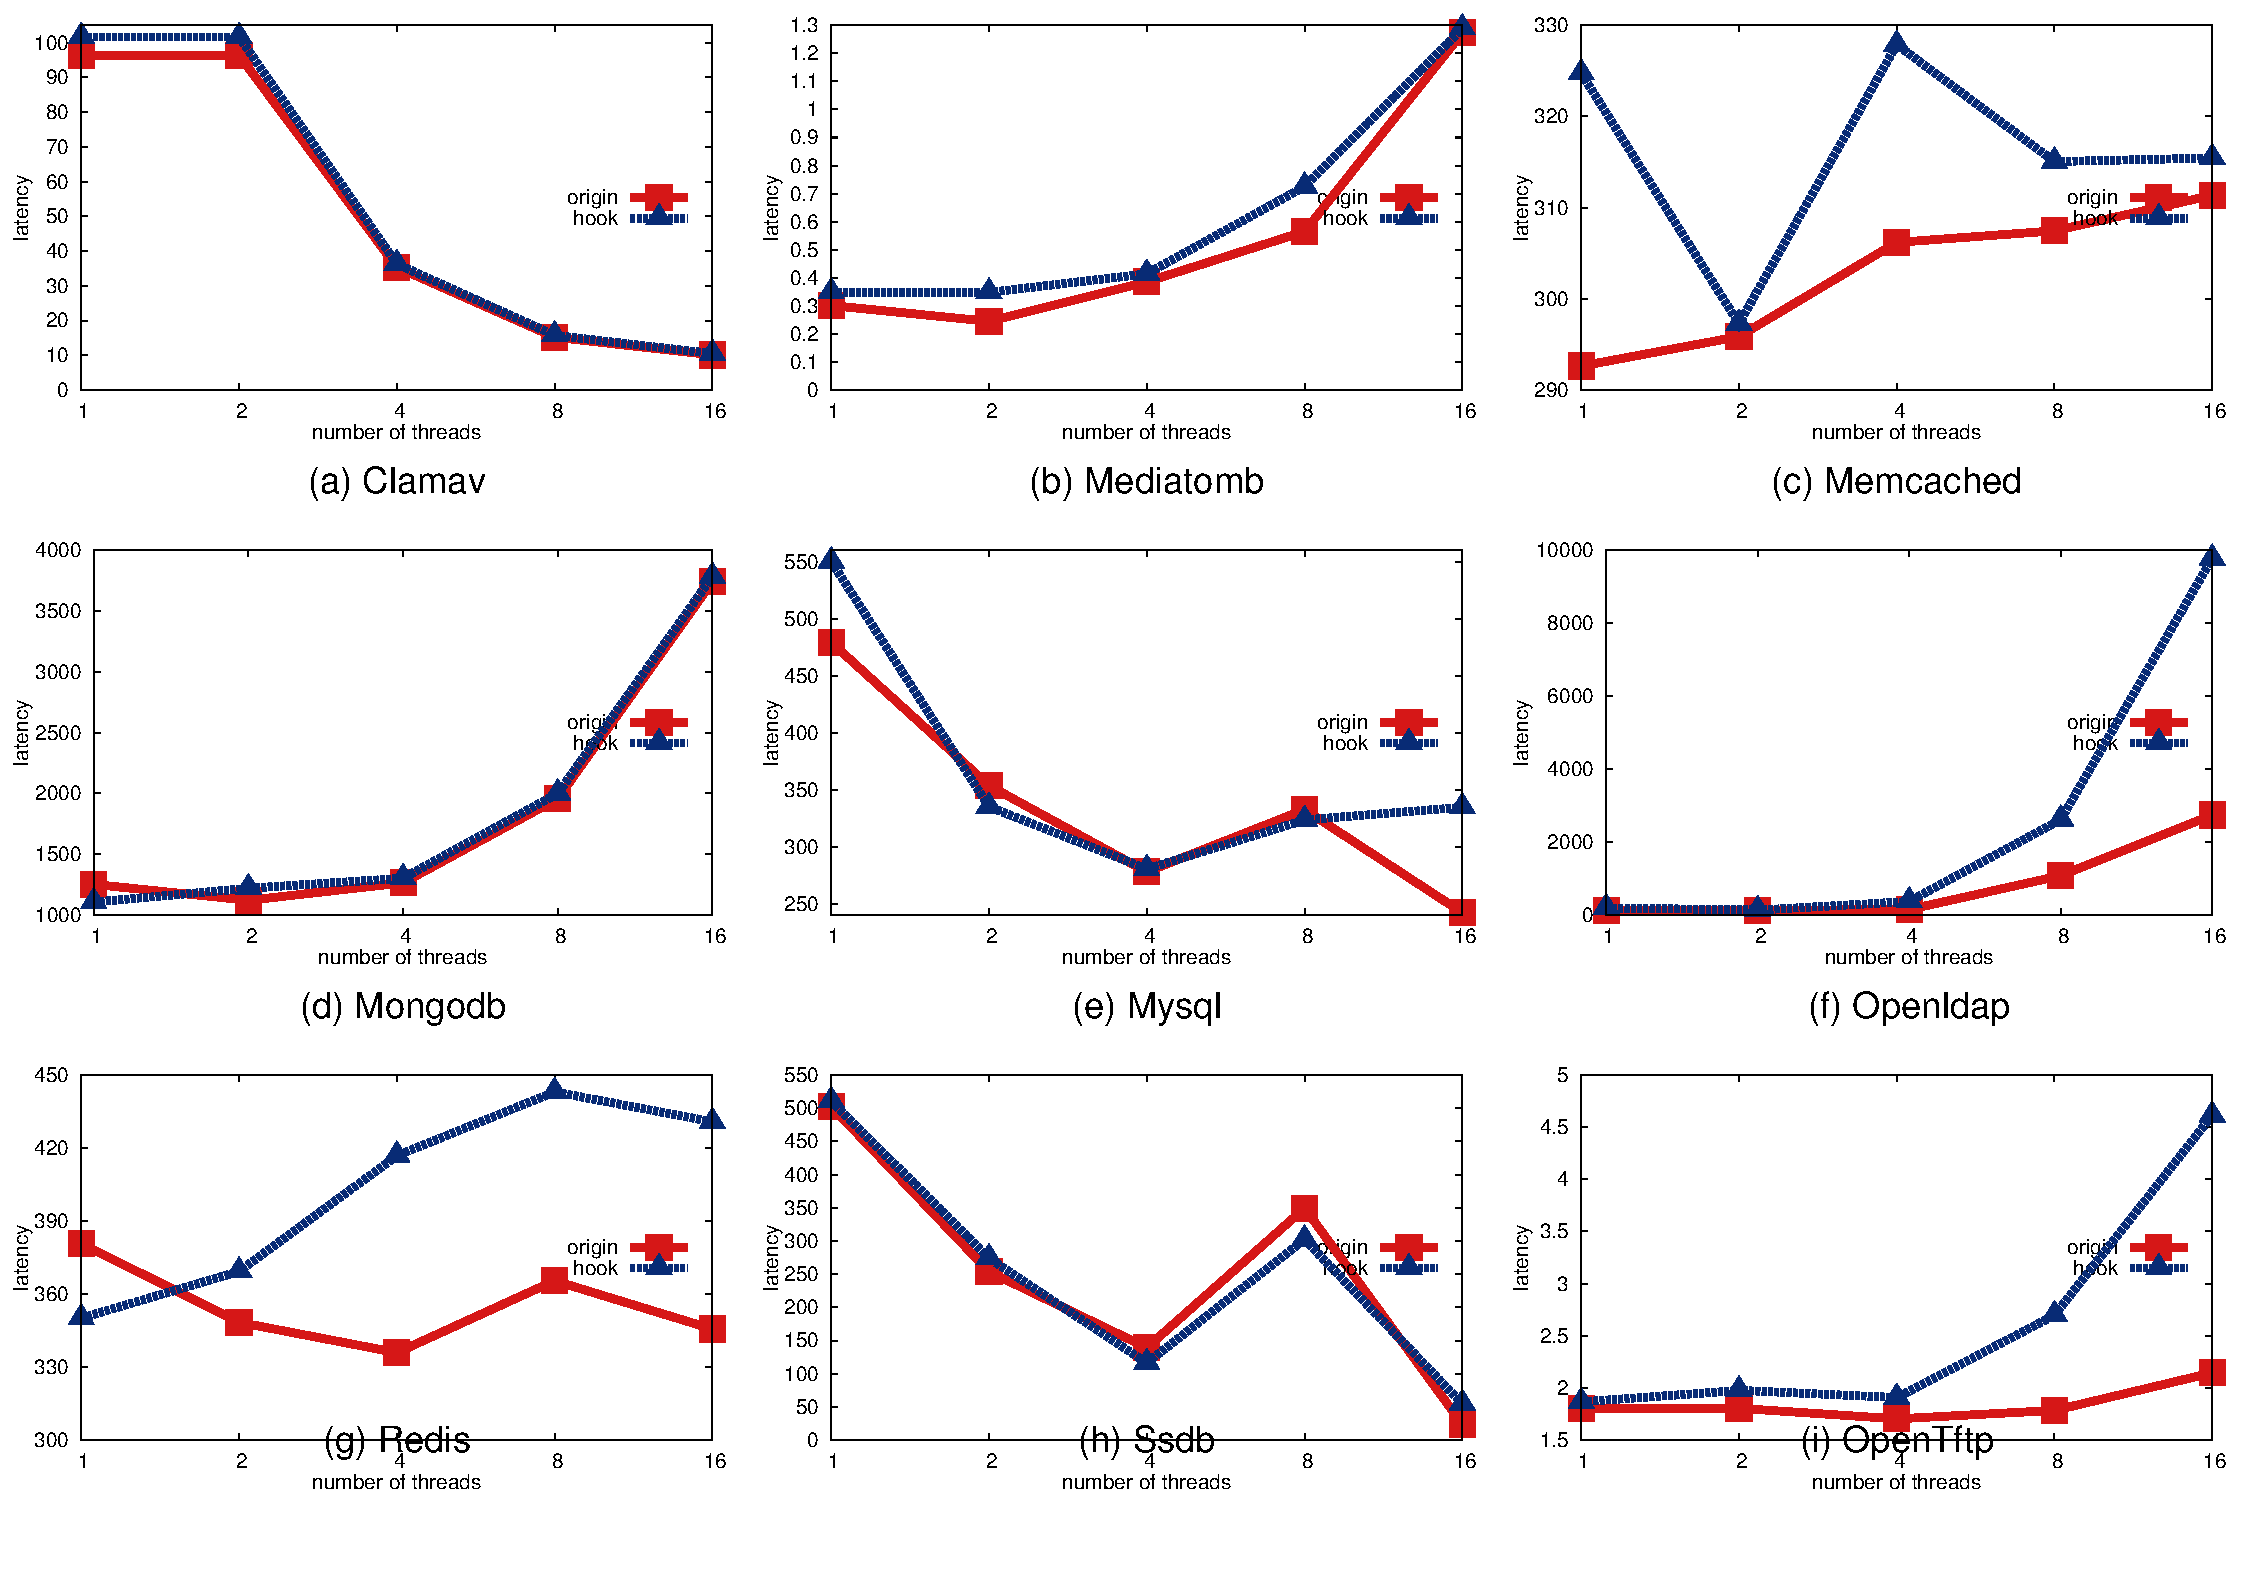
\includegraphics[width=0.9\textwidth]{figures/latency}
% \vspace{-.10in}
% \caption{\small {\em \xxx response time compared to the unreplicated
% execution.}}
% \vspace{-.20in}
% \label{fig:latency}
% \end{figure*}

To stress \xxx, we used a large replica group size of 9 to run all server 
programs. We spawned up to 32 concurrent connections, and then we measured both 
response 
time and throughput. We also measured \xxx's bare consensus latency. Each 
performance data point was taken from a mean value of 
10 executions.

% \subsection{Ease of Use} \label{sec:ease-of-use}

\xxx ran with \nprog evaluated programs without modifying them except
\calvin. \calvin integrates its client program and server program within the
same process and uses local memory to let these two programs talk. To
make \calvin's client and server communicate with POSIX sockets so that \xxx
can intercept the server's inputs, we wrote a \nlinescalvin-line patch for
\calvin.

We turned on and off the output checking (\S\ref{sec:output}) and didn't 
observe difference in \xxx performance. Only three programs (\mediatomb, 
\mysql, and \openldap) have different output hashes cause by physical times.

%  and Figure~\ref{fig:latency}
% response time
Figure~\ref{fig:tput} shows \xxx's throughput. We varied the number of 
concurrent client connections for each server program by from one to 32 
threads. For \calvin, we only collected the 8-thread result because \calvin 
uses this constant thread count in their code to serve client requests.

Overall, compared to these server programs' unreplicated executions, \xxx 
merely incurred a mean throughput overhead of \tputoverhead (note that in 
Figure~\ref{fig:tput}, the Y-axises of most programs start from a large 
number). As the number of threads increases, all programs' unreplicated 
executions got a performance improvement except \memcached. A prior
evaluation~\cite{rex:eurosys14} also observed a similar \memcached low
scalability. \xxx scaled almost as well as the unreplicated executions.
% a \latencyoverhead overhead compared to the unreplicated
% executions.

\xxx achieves such a low overhead in both throughput and response time mainly
because of two reasons. First, for each \recv call in a server, \xxx's input
coordination protocol only contains two one-sided RDMA writes and two efficient 
local SSD writes (\S\ref{sec:logging}) for the leader and each backup.

% A parallel SSD write
% approach~\cite{Bessani:usenix13} may further improve \xxx's SSD performance.
% Second, \xxx's output checking protocol invokes occasionally
% (\S\ref{sec:output-workflow}).

\begin{table}[h]
\footnotesize
\centering
\vspace{-.1in}
\begin{tabular}{lrrrr}
{\bf Program} & {\bf \# Calls} & {\bf Input} & {\bf SSD time}
& {\bf Quorum time}\\
\hline\\[-2.3ex]
% Heming: normalized clamav to 10K req.
\clamav & 30,000  & 37.0 & 7.9 \us & 10.9 \us\\
% TBD: normalize mediatomb to 10K req.
\mediatomb & 30,000  & 140.0 & 5.0 \us & 17.4 \us\\
\memcached & 10,016  & 38.0 & 4.9 \us & 7.0 \us\\
\mongodb & 10,376  & 490.6 & 7.8 \us & 9.2 \us\\
\mysql & 10,009  & 28.8 & 5.1 \us & 7.8 \us\\
% TBD: normalize ldap to 10K req.
\openldap & 10,016  & 27.3 & 5.5 \us & 6.4 \us\\
\redis & 10,016  & 40.5 & 2.8 \us & 6.3 \us\\
% TBD: normalize ssdb to 10K req.
\ssdb & 10,016  & 47.0 & 3.0 \us & 6.2 \us\\
\calvin & 10,002  & 128.0 & 8.7 \us  & 10.8 \us\\
\end{tabular}
\vspace{-.1in}
\caption{{\em Leader's input consensus events per 10K requests, 8 threads.}
The ``\# Calls" column means the number of socket calls that went through \xxx
input consensus; ``Input" means average bytes of a server's inputs received in
these calls; ``SSD time" means the average time spent on storing these calls to
stable storage; and ``Quorum time" means the average time spent on waiting
quorum.}
\vspace{-.1in}
\label{tab:consensus-latency}
\end{table}

% Figure~\ref{fig:latency} shows \xxx's latency.
% % Bare consensus latency, micro events.

To understand \xxx's performance overhead, we collected the number of
socket call events and consensus durations on the leader side.
Table~\ref{tab:consensus-latency} shows these statistics per 10K requests, 8
or max (if less than 8) threads. According to the consensus algorithm steps in
Figure~\ref{fig:consensus}, for each socket call, \xxx's leader does an ``L2":
SSD write (the ``SSD time" column in Table~\ref{tab:consensus-latency}) and an
``L4": quorum waiting phase (the ``quorum time" column). L4 implies backups'
performance because each backup stores the proposed socket call in local SSD and
then WRITEs a consensus reply to the leader.

By adding the last two columns in Table~\ref{tab:consensus-latency}, a 
\xxx input consensus took only 9.1 \us (\redis) to 22.4 \us (\mediatomb). 
% This consensus latency mainly depends on the ``Input" column: the average number of 
% data bytes received in socket calls (\eg, \mongodb has the largest received bytes).
\xxx's small consensus latency makes it achieve reasonable throughputs 
in Figure~\ref{fig:tput}. Overall, Figure~\ref{fig:compare} and 
Table~\ref{tab:consensus-latency}  indicate that \xxx has low overhead on 
server programs' response time. \xxx's mean overhead on response time was 
\latencyoverhead. Due to space limit, the response time overhead figure is put 
here~\cite{apus}.

% This small latency suggests that, even if clients are deployed within the same
% datacenter network, \xxx may still achieve acceptable overhead on many programs
% (although \xxx's deployment model is running server replicas in a datacenter and
% clients in LAN or WAN).

% \begin{table}[t]
% \footnotesize
% \centering
% % \vspace{-.2in}
% \begin{tabular}{lrr}
% {\bf Performance metric} & {\bf \zookeeper} & {\bf \xxx}\\
% \hline\\[-2.3ex]
% Throughput (requests/s) & 19,925   & 17,614 \\
% Consensus latency (\us) & 511.9  & 12.5\\
% \end{tabular}
% \vspace{-.1in}
% \caption{{\em Comparison with \calvin's \zookeeper replication.}}
% \vspace{-.2in}
% \label{tab:compare}
% \end{table}





% Comparison with Crane. Run Crane. TBD


% For seven nodes
% XXX TBD. We plan to buy more server machines for a larger scale of scalability
% evaluation.

% It
% would be interesting to see whether \xxx's scalability on replica group size is
% bounded by the outbound RDMA writes of RDMA NICs.



% Comparison with DARE. Three to five nodes.

\subsection{Checkpoint and Recovery} \label{sec:robust}

% \xxx's output checking protocol found different output results on \clamav,
% \openldap, and \mediatomb. The output divergence of \clamav was caused by its
% threading model: \clamav uses multiple threads to serve a directory scan
% request, where the threads scan files in parallel and append the scanned files
% into a shared output buffer protected by a mutex lock. Therefore, sometimes
% \clamav's output will diverge across replicas. Running a deterministic
% multithreading runtime with \clamav avoided this divergence~\cite{crane:sosp15}.
% \openldap and \mediatomb contained physical timestamps in their replies.
% \calvin did not send outputs to its client.

% TBD: what types of servers are good for output checking.

We ran the same performance benchmark as in \S\ref{sec:overhead} and measured 
programs' checkpoint timecost. Each \xxx periodic checkpoint operation 
(\S\ref{sec:checkpoint}) cost 0.12s to 11.6s on the evaluated server programs, 
depending on the amount of modified memory and files in the server programs 
since their own last checkpoint. \clamav incurred the largest checkpoint time 
(11.6s) because it loaded and scanned files in a \v{/lib} directory.

Checkpoint operations did not affect \xxx's performance in normal case because 
they were done on only one backup. The leader and other backups still formed 
majority and reached consensus rapidly.
% This indicates \paxos's fault-tolerance strength: a 
% backup restart or failure does not affect consensus. 

To evaluate \xxx's \paxos recovery feature, we ran \xxx with \redis and 
manually killed one backup, and we did not observe a performance change in the 
benchmark runs. We then manually killed the \xxx leader and measured the 
latency of our RDMA-based leader election with three rounds 
(\S\ref{sec:election}). Figure~\ref{tab:election} shows \xxx's election latency 
from three to eleven replicas. Because \paxos leader election is rarely 
invoked in practice, although \xxx's election latency was slightly higher than 
its normal case consensus latency, we considered it reasonable.

% efficiency of \xxx's rocovery, we ran \clamav and tried to randomly trigger its
% output divergence. \clamav's rocovery time varied from 1.47s to 1.49s for
% backups and the leader, including extracting files in its local directory,
% restoring process state with CRIU, and reconnecting RDMA QPs with remote
% replicas.



% Heming: TBD, just estimation. Current 0.81s to 2.72s are from redis.





\begin{table}[h]
\footnotesize
\centering
\vspace{-.05in}
\begin{tabular}{lrrrr}
{\bf \# Replicas} & {\bf 3} & {\bf 5} & {\bf 7} & {\bf 9}\\
\hline\\[-2.3ex]
Election latency (\us) & 10.7  & 12.0 & 12.8 & 13.5\\
\end{tabular}
\vspace{-.1in}
\caption{{\em \xxx's latency on on leader election.}}
\vspace{-.3in}
\label{tab:election}
\end{table}







% Once an output divergence is detected, \xxx will roll bacak the divergent
% replica, including leader and backups. For all the \nprog programs, our output
% checking protocol found these servers produced identical results except \clamav
% and \ssdb.
%
% \clamav's divergent output is caused by its special threading model:
% unlike the other evaluated programs which use one thread to server one client
% connection, \clamav uses multiple worker threads to serve a client request
% (\eg, scanning a directory path recursively). \xxx's worker threads
% concurrently contend for a global mutex lock and then append the scanned
% files into the output buffer for the client, causing a nondeterministic order
% of scanned files among all replicas. We manually compared \clamav's output
% across replicas, and we found the files were indeed the same except their order.
%
% We ran \ssdb on the same workload as in \S\ref{sec:overhead} and triggered a
% previous unkown concurrency bug in the QPUSH operations. This concurrency bug
% was triggered by concurrent client connections to push elements to a queue in
% \ssdb. In our evaluation, this bug was first triggered in a backup machine and
% caused a divergent output hash. the hashes of the other two replicas were
% still the same. \xxx's leader detected this divergence; it sent a
% rollback request to the divergent replica's guard, which took 1.2 \ms;
% the guard killed the \ssdb server and restored it from a prior
% checkpoint with 0.913 \ms, and the recovered replica reconnected to the other
% replicas and started to server requests in 0.09 \ms. Each process and file
% system checkpoint operation for \ssdb took 954 \ms.
%
% This minor divergence suggests that we hitted a bug, for two
% reasons. First, \xxx has enfored strongly consistent inputs across replicas, if
% only replicas diverge, this divergence must be caused by the server program
% itself, not different inputs. Second, only one replica diverged, this suggests
% that the output does not contain randome values (\eg, physical times, or the
% \clamav case), otherwise all replicas should diverged.
%
% We then carefully looked into the \ssdb source code and identified the bug. It
% was caused by incorrect synchronization to a global queue in \ssdb. We have
% reported this bug to the \ssdb developers with a suggested bug fixing
% patch~\cite{ssdb:bug}. Although \xxx does not intend to find bugs, this
% promising finding reflects that \xxx could be extended as an advanced testing
% tool: its fast, general SMR service lets it easily support general program, and
% its consistently enforce inputs and efficient output checking makes the minor
% replica output divergence a strong software bug indicator.
% Confidence. strongly consistent inputs.

%
% \subsection{Sensitivity of Parameters} \label{sec:sensitivity}

% Change output comparison periods. 1, 100, 1000, 10000. 1000 is the smallest
% number that starts to have negligible overhead. Run only with the server with
% largest recv() data size.

% Twait

% Tcomphash

% \subsection{Read-only Optimization} \label{sec:read-opt}

% %
